% =============================================================================
%  Romanization Flattens the Field
%  GlobalSouthAI @ NeurIPS 2026, non-archival workshop track.
%  Four-page short paper, written for this length rather than compressed.
%
%  COMPILER: pdfLaTeX.
%
%  Sinhala script: pdfLaTeX cannot set Sinhala, so the two inline Sinhala
%  snippets are drawn from PDF figures through \sinword. Until those files
%  exist the macro prints a visible grey placeholder. To switch it on, drop
%
%      figures/sin-kohomada.pdf   the single word "kohomada", used in S1
%      figures/sin-wesak.pdf      the three-word phrase romanized as
%                                 "wesak uthsawayeedii bauddhayin", used in S2
%
%  into place, cropped tight with no white margin, and change \sinhalafigsfalse
%  to \sinhalafigstrue below. Those are the only two slots in the paper.
%
%  Every number in this file is checked against the frozen analysis outputs by
%  paper/analysis/verify_claims.py.
% =============================================================================
\documentclass{article}

% Default: anonymous submission with line numbers, which is what double-blind
% review needs. Use [final] for a camera-ready version and [preprint] for a
% non-anonymous preprint.
\usepackage{neurips_2026}

\usepackage[utf8]{inputenc}
\usepackage[T1]{fontenc}
\usepackage{hyperref}
\usepackage{url}
\usepackage{booktabs}
\usepackage{amsfonts}
\usepackage{amsmath}
\usepackage{nicefrac}
\usepackage{microtype}
\usepackage{xcolor}
\usepackage{graphicx}

% ---- Sinhala inline words, as PDF images -------------------------------------
\newif\ifsinhalafigs
\sinhalafigsfalse
\newcommand{\sinword}[2]{%
  \ifsinhalafigs
    \raisebox{-0.25ex}{\includegraphics[height=2.0ex]{figures/#1}}%
  \else
    \colorbox{black!8}{\textcolor{black!55}{\scriptsize\texttt{[sin:#2]}}}%
  \fi}

% ---- helpers -----------------------------------------------------------------
\newcommand{\rom}[1]{\textit{#1}}
\newcommand{\bpb}{\textsc{bpb}}
\newcommand{\bpw}{\textsc{bpw}}
\newcommand{\mcc}{\textsc{mcc}}

% Float separation. The class default reserves 20pt above and below a float, which
% is generous for a paper whose figures sit at the top of the page. Text spacing,
% margins and font sizes are untouched.
\setlength{\textfloatsep}{15pt plus 2pt minus 4pt}
\setlength{\floatsep}{14pt plus 2pt minus 3pt}

% LaTeX's \input confuses the alignment scanner inside a tabular, so the
% machine-generated table bodies are pulled in with the TeX primitive instead.
\makeatletter
\newcommand{\rows}[1]{\@@input #1 }
\makeatother

% Anonymous placeholder. Replace before the camera-ready version. The
% transliterator is on PyPI, but naming the package would identify us.
\newcommand{\anonrepo}{\url{https://anonymous.4open.science/r/XXXXXXXX}}

\title{Romanization Flattens the Field: Script Variation\\and Metric Choice in
Sinhala Evaluation}

\author{%
  Anonymous Author(s)\\
  Affiliation\\
  Address\\
  \texttt{email}\\
}

\begin{document}
\maketitle

\begin{abstract}
Benchmarks for Global South languages are written in the formal script, while the
people who would use a model mostly type an ad hoc Romanized register in Latin
letters. We study that mismatch in Sinhala, an Indo-Aryan language with more than 17
million speakers. A recent
benchmark reported that language models are about 312 times worse on Romanized than on
Sinhala-script text, and that model scale predicts nothing. Re-measuring 31 checkpoints
with tokenizer-independent bits per byte, we reproduce the published perplexities and
split the reported ratio exactly in two: a factor of 21 is identical content being
cut into a different number of tokens, and a factor of 24 is a real rise in per-byte
loss. Under the corrected metric, scale does predict Sinhala-script ability. In the
first downstream evaluation of Sinhala script variation, 9{,}479 items and eleven
instruction-tuned checkpoints in both scripts for 208{,}538 generations, romanization
does not lower a field of models uniformly, it flattens it, and a 22.4 point spread in
Sinhala-script accuracy becomes 6.7 points. On offensive-language detection, accuracy
barely moves while Matthews correlation loses more than half its value. We close with
the evaluation practices this implies for other languages in the same position.
\end{abstract}

% =============================================================================
\section{Introduction}
\label{sec:intro}

Sinhala is an Indo-Aryan language written in a script of its own and spoken by more
than 17 million people, almost all of them in Sri Lanka
\citep{desilva-2019-survey, ranasinghe-etal-2025-sold}. Like several South Asian
languages it has an everyday orthographic split: formal writing uses the Sinhala
script, while comments, chat and social media are dominated by Romanized Sinhala,
known locally as Singlish and typed with Latin letters. It has no standard spelling, so
\sinword{sin-kohomada}{kohomada} (``how are you'') is typed \rom{kohomada},
\rom{kohomd} or \rom{kohomade} depending on the writer.

Every published Sinhala evaluation set we know of is in the Sinhala script. That is an
easily missed coverage gap, because the benchmark is in the right language and the wrong
register. Romanized registers persist for durable infrastructural reasons
rather than as a fashion \citep{sengupta-etal-2024-hinglish}, and in a deployed
maternal-health service \citet{khullar-etal-2025-scriptgap} found 83\% of Hindi and
73\% of Telugu user messages Romanized, with models handling them measurably worse.
Anyone serving Sinhala users is serving mostly Romanized input while validating on
Sinhala-script data.

\citet{rajapakse-weerasinghe-2026-script} measured that gap first, benchmarking 24
open-weight models with perplexity and reporting a median 312-fold degradation from
Sinhala-script to Romanized text and no correlation between parameter count and script
handling. Both numbers depend on the metric rather than on the models, because
perplexity is normalised by token count and token count for a fixed string is entirely
a property of the tokenizer \citep{gao-etal-2020-pile, magnusson-etal-2024-paloma}.
Sinhala is exactly where that matters, since tokenizers segment it very unevenly
\citep{petrov-etal-2023-tokenizers, ahia-etal-2023-languages}.

Recomputing tokenizer-independent bits per byte for 31 checkpoints splits the reported
ratio exactly in two, a factor of 21 from token-count normalisation and a factor of 24
from a real rise in per-byte loss, and the claim that scale does not help does not
survive (\S\ref{sec:metric}). In the first downstream evaluation of Sinhala script
variation, 9{,}479 items and 208{,}538 generations, romanization compresses the range of
model quality far more than it shifts the mean, turning a 22.4 point spread in accuracy
into 6.7 points (\S\ref{sec:flatten}). And on
offensive-language detection, accuracy falls a few points while Matthews correlation
loses more than half its value, so the metric decides whether the damage is visible at
all. None of this needed new models or new annotation, only a different denominator and
a competence screen. \S\ref{sec:lessons} states those as practices.

% =============================================================================
\section{Setup}
\label{sec:setup}

\paragraph{Data and conditions.} Every item is evaluated twice, in the Sinhala script as
published and in a Romanized form with identical content, so every comparison is paired
and differs only in orthography. The intrinsic corpus is the 500 parallel
sentence pairs of \citet{rajapakse-weerasinghe-2026-script}, whose Romanized side native
speakers typed, so the intrinsic results do not depend on our transliteration. Downstream we use every item of three sets with no sampling:
6{,}879 multiple-choice items from SinhalaMMLU \citep{pramodya-etal-2025-sinhalammlu},
where a mix of four and five option items puts guessing at 23.4\%, the
complete 2{,}500-item test split of the SOLD offensive-language task
\citep{ranasinghe-etal-2025-sold}, 40.6\% offensive so the majority class scores
59.4\%, and the 100 Sinhala items of Global PIQA \citep{chang-etal-2025-globalpiqa,
desilva-ranathunga-2026-sinhalapiqa}. That is 9{,}479 items over eleven
instruction-tuned checkpoints from 1.1B to 14.7B, or 208{,}538 zero-shot greedy
generations in 80 GPU hours, with one prompt template for every dataset so task and
prompt are not confounded. The intrinsic sweep covers 31 checkpoints from 350M to 14.7B,
24 of them prior work's pool (Appendix~\ref{sec:setupfull}).

\paragraph{The Romanized side.} Almost every Sinhala transliteration tool runs Latin
to Sinhala \citep{sumanathilaka-etal-2025-swabhasha} and we need the reverse, so we
wrote a deterministic grapheme-level transliterator using the digraph conventions
speakers actually type, turning \sinword{sin-wesak}{wesak uthsawayeedii bauddhayin}
into \rom{wesak uthsawayeedii bauddhayin}. Against 755{,}000 human-romanized reference
items it has the lowest character error rate of four methods, and 88.6\% of its
spellings are ones a human supplied for that word, against 84.2\% for the speakers who
typed the same sentences (Appendix~\ref{sec:translit}). It is released with the
evaluation harness and all analysis code at \anonrepo.

\paragraph{Statistics and the competence screen.} Paired comparisons use McNemar's test
\citep{mcnemar-1947} with Holm correction over checkpoints within a task
\citep{holm-1979}, and intervals come from 10{,}000 paired bootstrap resamples. A model
already at chance in the Sinhala-script condition cannot lose anything by being given
Romanized input, so averaging it in would understate the effect. We mark a checkpoint
\emph{competent} on a task when its Sinhala-script score beats the guessing baseline at
$p < 0.01$ under a Poisson-binomial null and it does not put more than 90\% of its
answers on one option. Six of eleven pass on SinhalaMMLU, six have a real signal on
SOLD, and none pass on Global PIQA.

% =============================================================================
\section{The Metric Was Measuring the Tokenizer}
\label{sec:metric}

Bits per byte divides total negative log-likelihood by a unit of the text itself rather
than by its tokenization, $\bpb = \sum_s \mathrm{NLL}(s) \,/\,
(\ln 2 \sum_s |s|_{\text{bytes}})$, and likewise per whitespace word, so the
denominator no longer depends on the vocabulary. Our recomputed perplexities reproduce
the published values to a median of 0.05\%, so what follows is the metric and not a
different run (Appendix~\ref{sec:reproduction}).

The two metrics disagree. Across the 31 checkpoints, Sinhala-script perplexity and bits
per byte are statistically unrelated ($\rho = 0.08$, $p = 0.68$), and Gemma-2-9B
ranks 26th of 31 on the first and 2nd on the second. Perplexity tracks tokenizer
fertility instead ($\rho = -0.87$, $p < 10^{-9}$), which runs from 4.3 tokens per
Sinhala word for the Qwen3.5 and Gemma tokenizers to 14.2 for models that fall back to
bytes, and spreading the same loss over three times as many tokens lowers perplexity
without the model knowing more.

That makes the reported ratio decomposable rather than arguable. Perplexity is
$\exp(\mathrm{NLL}/T)$ for $T$ scored tokens and $\mathrm{NLL} = \ln 2 \cdot A \cdot
B$ for $A$ bits per byte over $B$ bytes, so $\log_2 \mathrm{PPL} = A x$ with
$x = B/T$ the bytes each token carries, and the change across script conditions is
exactly
\begin{equation}
\Delta \log_2 \mathrm{PPL} =
\underbrace{\bar{A}\,(x_r - x_u)}_{\text{token-count normaliser}}
+ \underbrace{\bar{x}\,(A_r - A_u)}_{\text{per-byte loss}},
\label{eq:decomp}
\end{equation}
with $\bar{A}$ and $\bar{x}$ the two-condition means. The first term is identical
content being cut into a different number of tokens, the second the model genuinely
assigning less probability per byte. This is an identity rather than a model, and it
holds to $5 \times 10^{-15}$ bits in our data.

On prior work's 24 checkpoints the median gap is 8.29 bits, which is their 312-fold
ratio, and the split assigns 4.37 bits to the normaliser and 4.56 to per-byte loss, a
factor of 21 and a factor of 24 whose product is 312. Almost exactly half of the
headline is the unit of account, and the same measurement stated
tokenizer-independently is 2.14 bits per byte, a factor of 4.4. The scale claim reverses
too. Parameter count is uncorrelated with Sinhala-script perplexity
($\rho = 0.15$, $p = 0.42$) but correlated with Sinhala-script bits per byte
($\rho = -0.55$, $p = 0.001$), including on prior work's own 24 checkpoints
($\rho = -0.42$, $p = 0.04$). What scale does not buy is Romanized ability
($\rho = -0.28$, $p = 0.13$). Family, tokenizer and corpus vary together here, so that
is an association and not a scaling result.

% =============================================================================
\section{Romanization Flattens the Field}
\label{sec:flatten}

\begin{figure}[t]
\centering
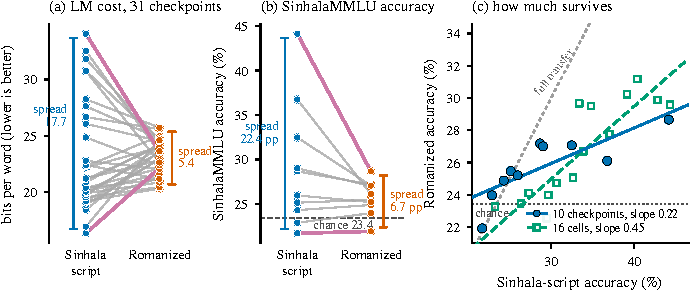
\includegraphics[width=0.94\linewidth]{figures/fig1_flattening.pdf}
\caption{(a) Language modelling cost. Word counts are identical within a pair, so the
columns are comparable, and the highlighted lines are checkpoints cheaper on Romanized
text. (b) SinhalaMMLU accuracy, where a 22.4 point spread becomes 6.7. (c) The same
numbers as levels, with the 16 domain by difficulty cells. Both slopes fall well below
the full-transfer slope of 1. LaMini-GPT-1.5B is omitted from (b) and (c) for
unparseable output on 95.9\% of Sinhala-script items.}
\label{fig:flat}
\end{figure}

Figure~\ref{fig:flat}(a) shows the effect that organises the rest. Sinhala-script cost
spans 16.3 to 34.1 bits per word across the 31 checkpoints while
Romanized cost collapses into a 20.3 to 25.7 band, and a full bit per word of
Sinhala-script improvement buys only 0.14 bits on Romanized text (95\% CI 0.05 to
0.25). Twelve of the 31 are \emph{cheaper} on Romanized text, and which ones is
predictable, because the better a checkpoint is on the Sinhala script the more it loses
($\rho = -0.88$, $p < 10^{-9}$). No checkpoint beats a held-out character bigram
on Romanized Sinhala, 3.06 bits per byte against 3.29 for the best of the 31 and 3.81
for the median (Appendix~\ref{sec:intrinsicfull}).

\paragraph{The same shape appears downstream.} Four of the six competent checkpoints
lose significantly on SinhalaMMLU after correction (Appendix
Table~\ref{tab:mainfull}), Qwen3.5-9B falling from 44.1\% to 28.7\% (95\% CI 14.0 to
16.9), and the two that lose least had 2.5 and 5.2 points of headroom.
Pooled, the gap is 6.0 points (95\% CI 5.4 to 6.5, $n = 41{,}274$).
Figure~\ref{fig:flat}(b) shows the levels, a 22.4 point Sinhala-script
spread becoming 6.7, with no checkpoint above 28.7\% against a 23.4\% chance baseline,
so the best one keeps 5.2 of its 20.7 points of headroom. Regressing Romanized on
Sinhala-script accuracy gives a slope of 0.22 (95\% bootstrap CI 0.11 to 0.54,
leave-one-out 0.17 to 0.26), reliably below the 1.0 of full transfer
($p = 8.6 \times 10^{-7}$) and above the 0.0 of total flattening. A refit over the
benchmark's 16 domain by difficulty cells, where the units are items, gives 0.45
(95\% CI 0.36 to 0.63).

\paragraph{On safety, accuracy hides it.} Accuracy on SOLD falls by 1.6 to 11.3 points
against a 59.4\% majority baseline, which looks survivable, while the median checkpoint
keeps only 45\% of its Matthews correlation. Five of the six lose significantly. The mechanism is a retreat toward triviality, and
Qwen2-7B-Instruct more than doubles its rate of predicting the offensive class, 10.5\%
to 23.4\%, without becoming more accurate. A deployment tracking accuracy would see a
five point wobble while over half the usable signal disappeared.

The effect is neither a tokenization artifact nor output degeneration. All eleven
checkpoints receive \emph{fewer} tokens in the Romanized condition on all three tasks, a
median 2.09 per word against 9.5 for the Sinhala script, and the invalid rate never exceeds 0.03\%
in either condition (Appendix~\ref{sec:extradetail}). The models keep answering across
the option set and are simply wrong.

% =============================================================================
\section{What This Means for Evaluating Global South Languages}
\label{sec:lessons}

Sinhala is one language, but the instruments that failed here are the ones in general
use and the conditions that made them fail are common.

\paragraph{Report a tokenizer-independent number.} A benchmark comparing perplexity
across model families, on a script those families tokenize unevenly, reports tokenizer
behaviour as much as model behaviour. Non-Latin and low-resource scripts are precisely
where fertility varies most \citep{petrov-etal-2023-tokenizers}, so for our languages
that is the default case and not a corner case. Bits per byte costs nothing extra on the same forward passes, and
here it moved a headline by a factor of 21.

\paragraph{A benchmark can be in the right language and the wrong script.} Coverage is
usually counted in languages, but for any language with a dominant Romanized register,
and Hindi, Telugu, Urdu, Nepali and Arabic dialects all qualify to some degree, a
language count overstates coverage of what users type. Building the second condition here needed a
transliterator in the direction almost no tooling supports, which is itself a reason
these registers stay unmeasured.

\paragraph{Screen for competence and state the guessing baseline.} Averaged over our
eleven checkpoints the script effect looks modest, because five of them are at or near
chance natively and contribute a zero gap by construction. For the same reason the hardest
strata reveal the smallest effects, 7.9 points on Easy items against 4.3 on Hard. Low-resource evaluation is full of near-chance results, so
unscreened group means understate script and dialect effects rather than overstate
them.

\paragraph{Choose a metric that survives class imbalance.} The safety task here is
40.6\% positive, so accuracy is anchored by the majority class. That is the normal
shape of moderation and triage data, and it is where a metric can look fine while the
system has stopped working.

\paragraph{The ranking you validate on is not the ranking you deploy.} Because
flattening is proportional to ability, the checkpoints that look best on Sinhala-script
benchmarks have the most to lose, and Romanized ability is nearly flat across a 42-fold
parameter range, so selecting on formal-script scores selects for the largest drop. The cheap quantity to log is absolute bits per byte, which tracks the downstream gap
($\rho = -0.83$, $n = 10$), and not the bits-per-byte \emph{gap}, which does not
($\rho = -0.15$, Appendix~\ref{sec:linkage}). The remedies are dull and available now:
transliterate before inference, put Romanized text in pretraining and instruction data,
and evaluate in the register you serve.

% =============================================================================
\section{Limitations}
\label{sec:limitations}

Everything here is one language, and the floor effect we describe may not transfer,
although \citet{khullar-etal-2025-scriptgap} report compatible magnitudes for six South
Asian languages. The Romanized side of the downstream items is transliterated rather
than human-typed, since no parallel resource exists at that scale. Rather than assume
that is neutral we measured it: our text is 0.17 to 0.24 bits per byte \emph{harder}
than what native speakers typed for the same sentences, so our gaps are closer to upper
bounds than to lower bounds. We cannot exclude Sinhala-script evaluation material in
pretraining, and everything is zero-shot on open weights up to 14.7B, so this is what a
user gets out of the box and not a ceiling. Appendix~\ref{sec:limitfull} has the rest.

% Marker for the page-budget check.
\label{sec:endofmain}

% =============================================================================
\bibliographystyle{plainnat}
\bibliography{custom}

\newpage
\appendix

% =============================================================================
\section{Related Work}
\label{sec:related}

\paragraph{Sinhala and low-resource evaluation.} Sinhala is low-resource and its
tooling has grown in a fragmented way \citep{desilva-2019-survey,
ranathunga-de-silva-2022-languages, joshi-etal-2020-state}. Recent resources are almost
entirely Sinhala-script: SinhalaMMLU \citep{pramodya-etal-2025-sinhalammlu}, SOLD
\citep{ranasinghe-etal-2025-sold}, the Sinhala split of Global PIQA
\citep{desilva-ranathunga-2026-sinhalapiqa, chang-etal-2025-globalpiqa} and encoder work
such as \citet{dhananjaya-etal-2022-bertifying}. The only benchmark treating script as a
variable is \citet{rajapakse-weerasinghe-2026-script}, which we extend.

\paragraph{Romanization gaps elsewhere.} Romanized South Asian text has been studied
mainly as a resource and identification problem \citep{roark-etal-2020-dakshina,
benton-etal-2025-improving}. \citet{j-etal-2024-romansetu} show romanization can
\emph{help} when models are adapted for it, the mirror image of our zero-shot setting.
The closest same-language work trains a model for the register:
\citet{chamikara-sumanathilaka-2026} fine-tune multilingual encoders for hate speech
detection on Romanized Sinhala, and \citet{hewapathirana-sumanathilaka-2024-emoscan}
build a classifier over Romanized Sinhala social media. We instead ask what
general-purpose generative models do out of the box. Closest in spirit is
\citet{khullar-etal-2025-scriptgap}, who find weighted F1 falling by as much as 24 points
on Romanized clinical queries. We add a paired item-level design with a competence
screen, a tokenizer-independent account of the same models, and a test of whether the gap
is a tokenization artifact.

\paragraph{Why not perplexity.} Bits per byte exists so that models with different
vocabularies can be compared \citep{gao-etal-2020-pile}, and Paloma adopts it for that
reason \citep{magnusson-etal-2024-paloma}. Tokenizers treat languages very unequally
\citep{petrov-etal-2023-tokenizers, ahia-etal-2023-languages} and over-segmentation costs
accuracy on low-resource tasks \citep{nag-etal-2024-fragmented}. To our knowledge ours is
the first work to show that the substantive conclusions of a published benchmark change
when the normaliser changes.

% =============================================================================
\section{Setup Details}
\label{sec:setupfull}

\paragraph{Hardware and compute.} The full study is roughly 80 hours of GPU wall
clock. The intrinsic sweep is about 10 hours over 46{,}500 scored sequences, and the
downstream run about 70 hours over 208{,}538 generations, of which roughly 25 hours
are Phi-4-14B alone. Inference is fp16 on two T4 GPUs, except Phi-4-14B which ran on
a single 16\,GB RTX 4070 Ti SUPER. The transliteration control of
\S\ref{sec:translit} adds 9{,}000 sequences in fp32 on 8 CPU cores in under an hour.
No training was performed at any point.

\paragraph{Prompting.} All prompts are zero-shot, greedily decoded with a 40-token
limit, and answers are extracted by pattern match with anything unparseable scored as
wrong. We chose one template from three candidates using a pilot of 3{,}240
generations over nine checkpoints, both script conditions and 20 items per dataset
(Table~\ref{tab:pilot}). The direct template won on SinhalaMMLU, the largest set, and
was the only candidate there that never produced unparseable output. An answer-first
template scored 1.4 points higher on SOLD and 7.2 higher on Global PIQA, and we
applied the direct template everywhere anyway, because a template chosen per dataset
would confound task with prompt, and because 20 items cannot resolve differences of
that size. What a paired comparison needs is not an optimal template but one that
does not favour a script, and the evidence for that is the main run, where the
unparseable rate never exceeds 0.03\% in either condition for the competent cohort
(Table~\ref{tab:invalidtau}). Twenty of the pilot's SinhalaMMLU items, 0.3\% of the
benchmark, are also in the final evaluation set.

\paragraph{Statistics.} Both conditions score the same items, so we use McNemar's
exact or continuity-corrected test \citep{mcnemar-1947, dror-etal-2018-hitchhikers}
and report discordant pair counts. Within each dataset we control the family-wise
error rate over checkpoints with Holm's procedure \citep{holm-1979}. Intervals on
gaps, macro-F1 differences, Matthews correlation differences and regression slopes
come from 10{,}000 paired bootstrap resamples over items, except for the
cross-checkpoint regressions of \S\ref{sec:flatten}, which resample checkpoints. For
SOLD we lead with Matthews correlation \citep{matthews-1975, chicco-jurman-2020}
because the classes are imbalanced and accuracy sits close to the majority baseline.
Item-level effects are also fitted as logistic regressions with checkpoint fixed
effects and cluster-robust standard errors by item, which put the odds ratio for
Romanized input on SinhalaMMLU at 0.70 ($p < 10^{-33}$) and give a significant
difficulty interaction ($p < 0.001$).

\begin{table}[t]
\centering\small
\setlength{\tabcolsep}{3.2pt}
\begin{tabular}{@{}lrrrrr@{}}
\toprule
& \multicolumn{3}{c}{\textbf{Accuracy \%}} & \multicolumn{2}{c}{\textbf{Invalid \%}} \\
\cmidrule(lr){2-4}\cmidrule(lr){5-6}
\textbf{Template} & S & R & both & S & R \\
\midrule
\rows{tables/tab_pilot.tex}
\bottomrule
\end{tabular}
\caption{The prompt-template pilot: 9 checkpoints, 3 templates, 2 script conditions,
20 items per dataset, 3{,}240 generations. Accuracy counts unparseable output as
wrong. T1 was applied to all three datasets even though T3 scored higher on SOLD and
Global PIQA, so that no dataset gets a different prompting regime. At 20 items per
dataset none of these differences is resolvable, which is why the pilot is treated as
a format check.}
\label{tab:pilot}
\end{table}

\begin{table}[t]
\centering\footnotesize
\setlength{\tabcolsep}{4pt}
\begin{tabular}{@{}lrlrr@{}}
\toprule
& & & \multicolumn{2}{c}{\textbf{tokens / word}} \\
\cmidrule(lr){4-5}
\textbf{Checkpoint} & \textbf{B} & \textbf{Hugging Face identifier}
& Sinh. & Rom. \\
\midrule
\rows{tables/tab_model_ids.tex}
\bottomrule
\end{tabular}
\caption{All evaluated checkpoints, with Hugging Face identifiers and tokenizer
fertility on the parallel corpus. $\ddagger$ marks the eleven used downstream and
$\bullet$ the 24 that \citet{rajapakse-weerasinghe-2026-script} evaluated.
Sinhala-script fertility varies by more than a factor of three across tokenizers,
whereas Romanized fertility is nearly constant.}
\label{tab:modelids}
\end{table}

% =============================================================================
\section{Reproducing the Published Benchmark}
\label{sec:reproduction}

Table~\ref{tab:shared24} sets our recomputation beside every headline number of
\citet{rajapakse-weerasinghe-2026-script} on its own 24 checkpoints. Per-checkpoint
absolute deviations from the published perplexities have a median of 0.05\% on
Sinhala-script text and 0.004\% on Romanized text, and 0.39\% on mixed-script text
once two outliers are excluded, Phi-4-14B and Mistral-Nemo-Base-2407. Everything in
\S\ref{sec:metric} is therefore the metric and not a different run.
Table~\ref{tab:decomp} applies Equation~\ref{eq:decomp} per checkpoint, and
Figure~\ref{fig:decomp} shows the same split as stacked bars.
Figure~\ref{fig:ppl} shows the disagreement between the two metrics directly.

Two details are worth stating. Over all 31 checkpoints the normaliser share of the
total falls to 39\%, and for the six Qwen3.5 and Gemma checkpoints the normaliser
term is slightly negative, because their tokenizers spend about the same number of
bytes per token in both scripts. Those six also hold the five smallest ratios in the
pool, with the four Qwen3.5 entries between 58-fold and 64-fold against a pool median
of 294-fold, so the eye-catching part of a 312-fold figure is concentrated in the
models whose tokenizers handle Sinhala worst. How completely the two metrics come
apart also depends on the pool: on the 24 published checkpoints the rank correlation
between perplexity and bits per byte is moderate ($\rho = 0.46$, $p = 0.02$), still
leaving four fifths of bits-per-byte rank variance unexplained, and adding the seven
newer checkpoints removes even that.

\begin{table}[t]
\centering\footnotesize
\setlength{\tabcolsep}{2.4pt}
\begin{tabular}{@{}lrr@{}}
\toprule
\textbf{Quantity} & \textbf{Published} & \textbf{Ours} \\
\midrule
\rows{tables/tab_shared24.tex}
\bottomrule
\end{tabular}
\caption{Our recomputation against the published benchmark, on its own 24
checkpoints. Deviations are per-checkpoint absolute percentage differences from the
published perplexities.}
\label{tab:shared24}
\end{table}

\begin{table}[t]
\centering\scriptsize
\setlength{\tabcolsep}{4pt}
\begin{tabular}{@{}lr r rr rr r@{}}
\toprule
& & & \multicolumn{2}{c}{\textbf{token-count normaliser}}
& \multicolumn{2}{c}{\textbf{per-byte loss}} & \\
\cmidrule(lr){4-5}\cmidrule(lr){6-7}
\textbf{Checkpoint} & \textbf{ratio} & \textbf{bits} & bits & factor & bits & factor
& \textbf{norm.\ \%} \\
\midrule
\rows{tables/tab_decomp.tex}
\bottomrule
\end{tabular}
\caption{Equation~\ref{eq:decomp} applied to every checkpoint, sorted by the reported
perplexity ratio. ``ratio'' is Romanized over Sinhala-script perplexity and ``bits''
its base-2 logarithm, which the two terms partition exactly. The last column is the
normaliser's share of the total, and $\bullet$ marks the 24 checkpoints of the
published pool.}
\label{tab:decomp}
\end{table}

\begin{figure}[t]
\centering
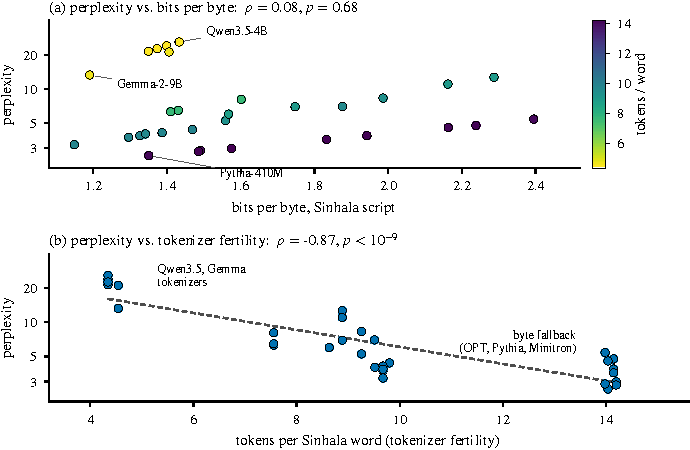
\includegraphics[width=\linewidth]{figures/fig2_perplexity_artifact.pdf}
\caption{(a) Sinhala-script perplexity against Sinhala-script bits per byte over 31
checkpoints. The two are unrelated ($\rho = 0.08$, $p = 0.68$). (b) Perplexity
against tokenizer fertility, which explains it almost fully ($\rho = -0.87$,
$p < 10^{-9}$).}
\label{fig:ppl}
\end{figure}

\begin{figure}[t]
\centering
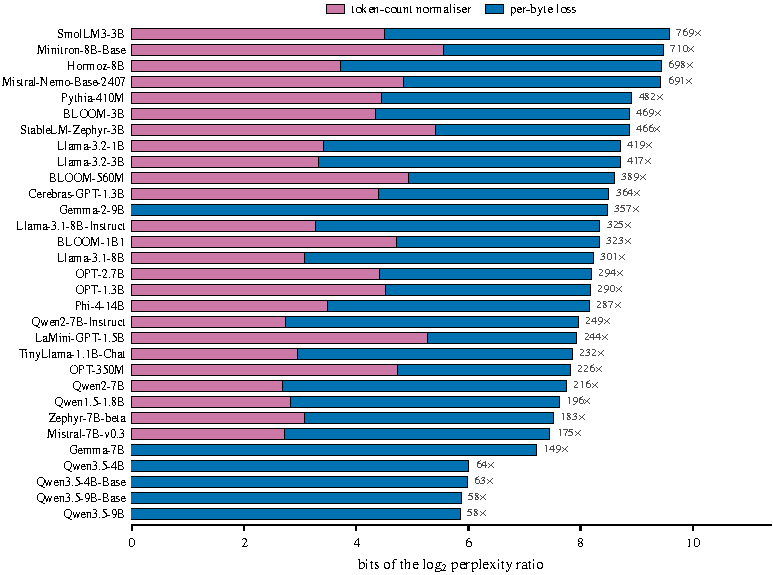
\includegraphics[width=\linewidth]{figures/fig5_ppl_decomposition.pdf}
\caption{The split of Equation~\ref{eq:decomp} per checkpoint. The two terms sum
exactly to the reported gap in bits.}
\label{fig:decomp}
\end{figure}

% =============================================================================
\section{Full Intrinsic Results}
\label{sec:intrinsicfull}

Table~\ref{tab:intrinsic} gives all 31 checkpoints, sorted by Sinhala-script bits per
byte. The two orderings disagree almost completely. Bits per word is the sharpest
cross-script unit, because a sentence and its romanization contain the same number of
words while Sinhala UTF-8 spends 2.65 bytes per character against 1.00 for Latin.

The mixed-script condition behaves quite differently from the Romanized one and
reproduces the earlier finding that script handling tracks general ability.
Sinhala-script and mixed-script bits per byte are strongly rank-correlated
($\rho = 0.94$) at a median gap of only 0.49 bits, against $\rho = 0.41$ for
Romanized. Interleaving scripts is a mild perturbation. Replacing one entirely is not.

Table~\ref{tab:ngram} gives the character $n$-gram reference points, fit on the same
corpus under five-fold cross-validation so every score is out of sample, and
Figure~\ref{fig:ngram} plots them against the checkpoints. On Romanized Sinhala the
best $n$-gram reaches 2.64 bits per byte and a character bigram 3.06, while the best
checkpoint reaches 3.29 and the median 3.81, so no checkpoint beats the bigram. On
the Sinhala script the picture is ordinary, with the character trigram at 1.16 and one
checkpoint below it. The $n$-gram is a cheap in-domain model and the comparison
favours it in that respect, so we read this as Romanized-condition checkpoints failing
to exploit structure beyond what a character bigram captures, rather than as a claim
about what they know. Two BLOOM checkpoints sit near the bottom of
Table~\ref{tab:intrinsic} on Sinhala-script text while being unremarkable on
Romanized text, and BLOOM is the only family in the pool with documented Sinhala
pretraining exposure \citep{lescao-etal-2023-bloom}.

\begin{table}[t]
\centering\scriptsize
\setlength{\tabcolsep}{3pt}
\begin{tabular}{@{}lr rrr rrr rr@{}}
\toprule
& & \multicolumn{3}{c}{\textbf{Sinhala script}}
& \multicolumn{3}{c}{\textbf{Romanized}}
& \multicolumn{2}{c}{\textbf{Mixed}} \\
\cmidrule(lr){3-5}\cmidrule(lr){6-8}\cmidrule(lr){9-10}
\textbf{Checkpoint} & \textbf{B} & PPL & \bpb{} & \bpw{}
& PPL & \bpb{} & \bpw{} & PPL & \bpb{} \\
\midrule
\rows{tables/tab_gs_intrinsic.tex}
\bottomrule
\end{tabular}
\caption{All 31 checkpoints, sorted by Sinhala-script bits per byte. $\ddagger$ marks
the eleven evaluated downstream. The perplexity and bits-per-byte orderings disagree
almost completely: Gemma-2-9B is 2nd by bits per byte and 26th by perplexity, and
Qwen3.5-9B-Base moves from 28th to 6th.}
\label{tab:intrinsic}
\end{table}

\begin{table}[t]
\centering\small
\setlength{\tabcolsep}{4pt}
\begin{tabular}{@{}lcccc@{}}
\toprule
& \multicolumn{2}{c}{\textbf{Sinhala script}} & \multicolumn{2}{c}{\textbf{Romanized}} \\
\cmidrule(lr){2-3}\cmidrule(lr){4-5}
\textbf{Model} & \bpb{} & \#\,LMs $<$ & \bpb{} & \#\,LMs $<$ \\
\midrule
\rows{tables/tab_ngram.tex}
\bottomrule
\end{tabular}
\caption{Held-out add-1 character $n$-gram models against the 31 checkpoints,
five-fold cross-validated so every score is out of sample. ``\#\,LMs $<$'' counts
checkpoints achieving lower bits per byte than the $n$-gram model.}
\label{tab:ngram}
\end{table}

\begin{figure}[t]
\centering
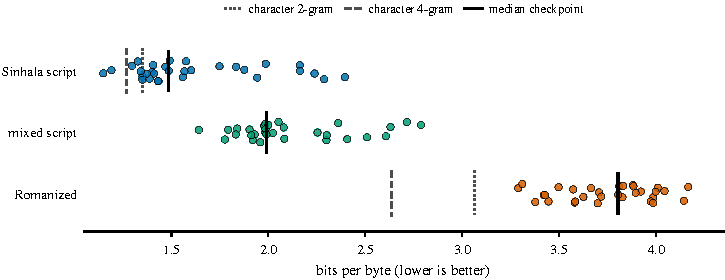
\includegraphics[width=\linewidth]{figures/fig4_ngram_reference.pdf}
\caption{Checkpoint bits per byte against character $n$-gram references in both
conditions. On Romanized Sinhala every checkpoint sits above the bigram.}
\label{fig:ngram}
\end{figure}

% =============================================================================
\section{Full Downstream Results}
\label{sec:extradetail}

Table~\ref{tab:mainfull} gives all eleven checkpoints on SinhalaMMLU and SOLD, with
macro-F1 alongside Matthews correlation.
Table~\ref{tab:strata} breaks SinhalaMMLU into difficulty and domain strata pooled
over the six competent checkpoints, Table~\ref{tab:piqa} gives Global PIQA per
checkpoint, and Table~\ref{tab:invalidtau} gives the two controls of
\S\ref{sec:flatten} per checkpoint, the unparseable rates and the ratio of Romanized
to Sinhala-script input tokens. Figure~\ref{fig:sold} shows the SOLD result, where
accuracy and Matthews correlation disagree about whether anything happened.

Two numbers in Table~\ref{tab:mainfull} are worth flagging. LaMini-GPT-1.5B and
TinyLlama-1.1B-Chat appear to improve under romanization, and both are artifacts of
their failing to produce parseable output on the Sinhala-script side rather than script
effects, which is what the competence screen exists to catch. The SOLD offensive-class
rates behind the retreat toward triviality are 10.5\% to 23.4\% for Qwen2-7B-Instruct
and 9.8\% to 20.7\% for Hormoz-8B.

\begin{table}[t]
\centering\scriptsize
\setlength{\tabcolsep}{2.6pt}
\begin{tabular}{@{}lr rrr l r rr rr r@{}}
\toprule
& & \multicolumn{5}{c}{\textbf{SinhalaMMLU} (6{,}879 items)}
& \multicolumn{5}{c}{\textbf{SOLD} (2{,}500 items)} \\
\cmidrule(lr){3-7}\cmidrule(lr){8-12}
& & \multicolumn{2}{c}{Acc.\ \%} & & &
& \multicolumn{2}{c}{macro-F1} & \multicolumn{2}{c}{\mcc} & \\
\textbf{Checkpoint} & \textbf{B} & S & R & $\Delta$ & 95\% CI & $p_{\text{Holm}}$
& S & R & S & R & $p_{\text{Holm}}$ \\
\midrule
\rows{tables/tab_extrinsic_main.tex}
\bottomrule
\end{tabular}
\caption{All eleven downstream checkpoints, ordered by size. S is the Sinhala script,
R is Romanized, $\Delta$ is the paired difference in points, $p_{\text{Holm}}$ is
McNemar's test corrected across checkpoints within a task, and $\mcc$ is Matthews
correlation with a paired-bootstrap $p$. $\dagger$ marks checkpoints passing the
competence screen.}
\label{tab:mainfull}
\end{table}

\begin{table}[t]
\centering\small
\setlength{\tabcolsep}{4pt}
\begin{tabular}{@{}lrrrrr@{}}
\toprule
\textbf{Stratum} & \textbf{Items} & \textbf{S \%} & \textbf{R \%}
& \boldmath$\Delta$ & \boldmath$p_{\text{Holm}}$ \\
\midrule
\rows{tables/tab_strata.tex}
\bottomrule
\end{tabular}
\caption{SinhalaMMLU by stratum, pooled over the six competent checkpoints. Item
counts are per checkpoint and domains are ordered by loss.}
\label{tab:strata}
\end{table}

\begin{table}[t]
\centering\small
\setlength{\tabcolsep}{3.4pt}
\begin{tabular}{@{}lrrrcr@{}}
\toprule
& \multicolumn{2}{c}{Acc.\ \%} & & \textbf{disc.} & \\
\cmidrule(lr){2-3}\cmidrule(lr){5-5}
\textbf{Checkpoint} & S & R & \boldmath$\Delta$ & \textbf{b/c}
& \boldmath$p_{\text{Holm}}$ \\
\midrule
\rows{tables/tab_piqa.tex}
\bottomrule
\end{tabular}
\caption{Global PIQA, 100 items. ``disc.\ b/c'' are the discordant pair counts
entering McNemar's test. No checkpoint is above chance in the Sinhala-script
condition and no comparison survives correction, so we treat this task as
underpowered rather than as corroboration.}
\label{tab:piqa}
\end{table}

\begin{table}[t]
\centering\small
\setlength{\tabcolsep}{3.2pt}
\begin{tabular}{@{}lrrrrr@{}}
\toprule
& \multicolumn{2}{c}{\textbf{MMLU inv.\ \%}} & \multicolumn{2}{c}{\textbf{PIQA inv.\ \%}} & \\
\cmidrule(lr){2-3}\cmidrule(lr){4-5}
\textbf{Checkpoint} & S & R & S & R & \boldmath$\tau$ \\
\midrule
\rows{tables/tab_invalid_tau.tex}
\bottomrule
\end{tabular}
\caption{Unparseable-output rates, and $\tau$, the ratio of Romanized to
Sinhala-script input tokens on SinhalaMMLU. $\tau$ is below one for every checkpoint,
so the Romanized condition is the shorter input in every case.}
\label{tab:invalidtau}
\end{table}

\begin{figure}[t]
\centering
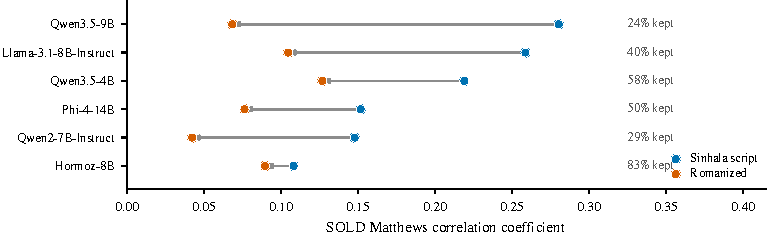
\includegraphics[width=\linewidth]{figures/fig3_sold_mcc.pdf}
\caption{SOLD under romanization. Accuracy moves a few points against a 59.4\%
majority baseline while Matthews correlation loses a median 55\% of its value.}
\label{fig:sold}
\end{figure}

% =============================================================================
\section{Every Refit of the Flattening Regressions}
\label{sec:flattenfull}

Table~\ref{tab:flatten} lists every fit. One deserves explanation, because it is the
natural way to state the result and it is a trap. Writing headroom as Sinhala-script
accuracy minus chance, the paired loss fits headroom at
$\text{loss} = 0.78 \times \text{headroom} - 1.06$ with $R^2 = 0.96$. But
Sinhala-script accuracy appears on both axes, so a high fit is close to guaranteed.
Shuffling the Romanized scores to destroy any association still yields a mean slope of
1.00 and a mean $R^2$ of 0.94, with 8.9\% of permutations reaching
$R^2 \geq 0.96$. We do not treat that fit as evidence, and we report it here because
the same construction is easy to reach for in any robustness study. The levels form we
do rely on returns a mean slope of 0.00 and a mean $R^2$ of 0.11 under the same null,
and only 0.5\% of permutations reach the observed fit. The cell-level refit is 0.48
when cells are weighted by item count. The two views are complementary rather than
independent, since they aggregate the same generations differently, but they agree on
the shape and disagree usefully on the amount: content-level transfer is about twice
model-level transfer.

\begin{table}[t]
\centering\footnotesize
\setlength{\tabcolsep}{2pt}
\begin{tabular}{@{}lr@{}}
\toprule
\textbf{Fit} & \textbf{Value} \\
\midrule
\rows{tables/tab_flatten.tex}
\bottomrule
\end{tabular}
\caption{Every refit of the two flattening regressions. The levels form regresses
Romanized on Sinhala-script accuracy. The headroom form regresses the paired loss on
Sinhala-script headroom above chance and is reported only to show why we do not rely
on it.}
\label{tab:flatten}
\end{table}

% =============================================================================
\section{Do Intrinsic Metrics Track Downstream Fragility?}
\label{sec:linkage}

For the ten checkpoints measured both ways, absolute Sinhala-script bits per byte
tracks the SinhalaMMLU gap ($\rho = -0.83$, 95\% CI $-1.00$ to $-0.30$,
leave-one-out $-0.90$ to $-0.77$) and the loss of Matthews correlation on SOLD
($\rho = -0.78$, CI $-1.00$ to $-0.36$, leave-one-out $-0.87$ to $-0.73$), which is
the flattening of \S\ref{sec:flatten} seen from the intrinsic side. The negative
result is the more useful one. The bits-per-byte \emph{gap}, the natural analogue of
the degradation ratio prior work reports, shows no association ($\rho = -0.15$, CI
$-0.89$ to $+0.63$), and neither does the perplexity ratio ($\rho = -0.52$). For the
gap even the leave-one-out range straddles zero, so we cannot sign it.

All of this is exploratory: ten heterogeneous checkpoints, no held-out validation, no
pre-registration, and intervals wide enough to reach $-1.00$. The levels-versus-gaps
contrast is stable under leave-one-out, but Table~\ref{tab:linkage} is a hypothesis
for a larger checkpoint set rather than a screening instrument.

\begin{table}[t]
\centering\small
\setlength{\tabcolsep}{3pt}
\begin{tabular}{@{}l r@{~}l r@{~}l@{}}
\toprule
& \multicolumn{2}{c}{\textbf{MMLU gap}} & \multicolumn{2}{c}{\textbf{SOLD} $\Delta\mcc$} \\
\cmidrule(lr){2-3}\cmidrule(lr){4-5}
\textbf{Intrinsic predictor} & $\rho$ & 95\% CI & $\rho$ & 95\% CI \\
\midrule
\rows{tables/tab_linkage.tex}
\bottomrule
\end{tabular}
\caption{Spearman correlations between intrinsic measurements and downstream script
effects, over the ten parseable checkpoints, with bootstrap intervals. Levels track
the effect, gaps and ratios do not. The intervals are wide because $n = 10$, which is
why this is exploratory.}
\label{tab:linkage}
\end{table}

% =============================================================================
\section{The Transliterator, and What It Costs}
\label{sec:translit}

Our transliterator is a deterministic grapheme-level converter that parses Sinhala as
an abugida and uses the digraph conventions speakers type rather than a scholarly
scheme, so the dental stop becomes \rom{th} and the labiodental approximant becomes
\rom{w}. It runs locally, covers every input, and collapses only the consonant
distinctions casual Singlish also collapses.

\paragraph{Against human references.} We validated it on 755{,}000 human-romanized
items from the Swa-bhasha Resource Hub \citep{sumanathilaka-etal-2025-swabhasha}:
4{,}397 authentic social-media sentence pairs, 450{,}587 words each carrying several
accepted spellings, and a 300{,}000-sentence machine-augmented cross-check. Scored
against the closest accepted reference by character error rate, chrF
\citep{popovic-2015-chrf} and exact match, ours has the lowest error rate of four
methods on all three corpora, 0.182, 0.121 and 0.112, and a paired Wilcoxon test
separates it from Aksharamukha \citep{rajan-aksharamukha}, uroman
\citep{hermjakob-etal-2018-uroman} and the web romanizer of
\citet{desilva-ranathunga-2026-sinhalapiqa} at $p < 10^{-90}$ on the two large
corpora (Table~\ref{tab:methods}). The residual difference from human typing is one
convention rather than phonemic error. All four methods double long vowels far more
often than people do, 0.81 per word against 0.12. Word by word against the
human-typed side of the parallel corpus, 44.6\% of our forms match exactly and a
further 27.6\% match once that convention is normalised, leaving 27.8\% residual, and
against the multi-reference lexicon of 449{,}598 words and 7{,}075{,}844 spellings,
88.6\% of our spellings are ones a human actually supplied for that word, against
84.2\% for the native speakers who typed the same sentences
(Tables~\ref{tab:attest} and \ref{tab:mismatch}).

\paragraph{What the substitution costs a model.} The Romanized side of the downstream
items is ours rather than human-typed, so we measured what that substitution costs.
On the 500 parallel sentences, whose Romanized side native speakers typed, our text
is 0.174 to 0.240 bits per byte harder than theirs, positive for all six checkpoints
we could rerun, with a median of 0.219 (Table~\ref{tab:svh}). Our condition is
therefore somewhat harder than authentic typing, which makes the downstream gaps we
report closer to upper bounds than to lower bounds. This cuts against what the
spelling statistics alone would suggest, and we report it because it bounds the claim
rather than because it helps it. Two things limit how far that control carries. It
covers six of 31 checkpoints, all below 3.2B parameters, and none of the six passes
the downstream competence screen. For the checkpoints that do carry the downstream
result we instead test the same worry item by item on SOLD, and find that how closely
an item's Romanized spellings match attested human spellings does not predict its
Romanized penalty, with a Spearman correlation of $0.02$ ($p = 0.31$, $n = 2{,}447$)
and terciles losing 5.0, 7.2 and 7.3 points from least to most attested
(Table~\ref{tab:attesttercile}). The intrinsic results do not share this limitation at
all, since their Romanized side was typed by native speakers, and they show the same
flattening. A human-written Romanized version of even a few hundred SinhalaMMLU items
would still settle the question better than any of this.

\begin{table}[t]
\centering\small
\setlength{\tabcolsep}{2.2pt}
\begin{tabular}{@{}lccccc c@{}}
\toprule
& \multicolumn{3}{c}{\textbf{CER} $\downarrow$} & \textbf{chrF} & \textbf{Exact} & \textbf{Cov.} \\
\cmidrule(lr){2-4}\cmidrule(lr){5-5}\cmidrule(lr){6-6}\cmidrule(lr){7-7}
\textbf{Method} & sent. & word & aug. & sent. & word & \% \\
\midrule
\rows{tables/tab_methods.tex}
\bottomrule
\end{tabular}
\caption{Transliteration quality against human references: 4{,}397 authentic
social-media sentence pairs, 450{,}587 multi-reference words, and a fixed
300{,}000-sentence sample of a machine-augmented set. Coverage is the share of inputs
the method produced any output for.}
\label{tab:methods}
\end{table}

\begin{table}[t]
\centering\footnotesize
\setlength{\tabcolsep}{2.4pt}
\begin{tabular}{@{}lrrrr@{}}
\toprule
& & & \multicolumn{2}{c}{\textbf{attested \%}} \\
\cmidrule(lr){4-5}
\textbf{Text} & \textbf{tokens} & \textbf{cov.\ \%} & raw & norm. \\
\midrule
\rows{tables/tab_attest.tex}
\bottomrule
\end{tabular}
\caption{Share of word tokens whose Romanized spelling is one a human supplied for
that Sinhala word in the Swa-bhasha lexicon. ``tokens'' counts the word tokens the
lexicon covers and ``cov.'' the share of all Sinhala word tokens that is. ``norm.''
collapses runs of the same Latin vowel on both sides. The first row is the reference
point: it applies the same measure to text native speakers typed.}
\label{tab:attest}
\end{table}

\begin{table}[t]
\centering\small
\begin{tabular}{@{}llr@{}}
\toprule
\textbf{Ours} & \textbf{Human} & \textbf{n} \\
\midrule
\rows{tables/tab_mismatch.tex}
\bottomrule
\end{tabular}
\caption{The twelve most frequent word-level disagreements with the human-typed side
of the parallel corpus that survive normalising the long-vowel convention. Most are
vowel reduction or abbreviation on the human side.}
\label{tab:mismatch}
\end{table}

\begin{table}[t]
\centering\scriptsize
\setlength{\tabcolsep}{2.6pt}
\begin{tabular}{@{}lr rrr rr@{}}
\toprule
& & \multicolumn{3}{c}{\textbf{bits per byte}} & & \textbf{PPL} \\
\cmidrule(lr){3-5}
\textbf{Checkpoint} & \textbf{B} & Sinh. & human & ours
& \boldmath$\Delta$ & ratio \\
\midrule
\rows{tables/tab_svh.tex}
\bottomrule
\end{tabular}
\caption{Our transliteration against human typing on the same 500 sentences.
$\Delta$ is ours minus human bits per byte, positive meaning our text is harder.
``PPL ratio'' is our perplexity over the human perplexity, below one for every
checkpoint even though bits per byte is higher, because our spellings occupy more
tokens. The Sinhala-script and human columns reproduce the recorded run to within
0.11\%. $\ddagger$ marks checkpoints also evaluated downstream. Six of 31
checkpoints, all below 3.2B and none passing the competence screen, so this bounds
the direction rather than settling it.}
\label{tab:svh}
\end{table}

\begin{table}[t]
\centering\small
\setlength{\tabcolsep}{2.8pt}
\begin{tabular}{@{}lrr rrr l@{}}
\toprule
\textbf{Attest.} & \textbf{items} & \textbf{att.\ \%}
& \textbf{S \%} & \textbf{R \%} & \boldmath$\Delta$ & \textbf{95\% CI} \\
\midrule
\rows{tables/tab_attest_tercile.tex}
\bottomrule
\end{tabular}
\caption{SOLD items split into terciles by how often their Romanized spellings are
attested in the human lexicon, pooled over the five competent checkpoints. If our
transliterator's idiosyncrasies drove the Romanized penalty, the low-attestation
tercile would lose most. It loses least. The tercile with the smallest gap also has
the lowest Sinhala-script accuracy, which the flattening of \S\ref{sec:flatten}
already predicts.}
\label{tab:attesttercile}
\end{table}

% =============================================================================
\section{Full Limitations}
\label{sec:limitfull}

\paragraph{One language.} Everything here is Sinhala. The mechanism we describe, a
floor effect that makes robustness gaps proportional to formal-script ability, should
generalise to any language with a dominant Romanized register, but we have not shown
that. Hindi, Nepali, Telugu, Urdu, Tamil and Arabic dialects are the obvious tests,
and \citet{khullar-etal-2025-scriptgap} report compatible magnitudes for Hindi,
Nepali, Telugu, Kannada, Marathi and Punjabi.

\paragraph{The Romanized side of the downstream sets is synthetic.} See
\S\ref{sec:translit}. We transliterate rather than collect human-typed Romanized
versions, because no such parallel resource exists at this scale, and we measured
that our text is the harder end of the range rather than assuming it is neutral.

\paragraph{Checkpoint size is confounded with everything else.} Our 31 checkpoints
differ in family, tokenizer, training corpus and instruction-tuning status at the
same time. The association between parameter count and Sinhala-script bits per byte
is not a scaling law, and our own fertility analysis is direct evidence that
family-level confounds are present.

\paragraph{We cannot exclude contamination.} The training corpora of these
checkpoints are not fully auditable, so we cannot rule out that public evaluation
sets, or Sinhala-script material closely related to them, appeared during
pretraining. If they did, the Sinhala-script side would be inflated and the gaps we
report overstated. This applies to any evaluation of pretrained models on public
benchmarks and we have no way to bound it here.

\paragraph{The intrinsic-to-downstream link is exploratory.} Ten checkpoints, no
held-out validation, no pre-registration, and bootstrap intervals wide enough to
reach $-1.00$ (\S\ref{sec:linkage}).

\paragraph{The mixed-script condition is weaker evidence than the rest.} That corpus
is authentic mixed-script text rather than a transliteration of the parallel set, so
it is not parallel to either script condition. It supports a descriptive statement
about how mildly script mixing perturbs cost, and nothing paired.

\paragraph{Open weights only, and small ones.} We evaluate open checkpoints up to
14.7B downstream. Frontier proprietary models are much stronger on Sinhala
\citep{pramodya-etal-2025-sinhalammlu} and therefore have far more headroom, so the
flattening slope predicts larger absolute losses for them. That prediction is
untested here.

\paragraph{Zero-shot only.} One template, zero-shot, greedy. This measures what a
user gets out of the box, not the ceiling. Few-shot prompting,
transliterate-then-infer, or Romanized fine-tuning could all narrow the gap, and we
do not measure by how much.

\paragraph{Two checkpoints cannot do the task.} LaMini-GPT-1.5B and
TinyLlama-1.1B-Chat produce unparseable output on most Sinhala-script items of at
least one task. Their apparent improvement under romanization is an artifact of that
failure, not a script effect, which is why the competence screen exists.

% =============================================================================
\section{Ethics}
\label{sec:ethics}

\paragraph{Content warning.} \S\ref{sec:flatten} and
Appendix~\ref{sec:extradetail} discuss an offensive-language dataset. We quote no
offensive text anywhere in this paper and report only aggregate metrics over it.

\paragraph{Data.} All datasets are public research releases used for evaluation only.
Global PIQA forbids training on it or on synthetic data seeded from it, and we do
neither. SinhalaMMLU is released under a licence that forbids distributing
adaptations, and its authors asked that the full set not be made public, so our
Romanized version of it stays local. SOLD contains offensive social media text,
already pseudonymised upstream with user mentions replaced by placeholders, and we
neither collected nor re-annotated any of it. We add no new human annotation and no
new data collection, so no ethics approval was required.

\paragraph{Models.} All 31 checkpoints were used for evaluation only, with no
fine-tuning, redistribution or derivative model release, which is within the terms of
each family's licence, including the Llama Community License, the Gemma Terms of Use
and the BigScience RAIL licence.

\paragraph{Risk.} The practical risk our results speak to is deployment. A moderation
or support system validated on Sinhala-script text and serving Romanized users will
look far better in evaluation than in the field, and on SOLD that failure is invisible
in accuracy while more than half the usable signal is gone. Publishing the size of
that gap, and a screen that stops averaging from hiding it, is the useful response.
Our transliterator collapses several Sinhala consonant distinctions, matching casual
Singlish practice, so it is a tool for building evaluation data and not for rendering
names or other text where those distinctions carry meaning.

% =============================================================================
\section{Licences and Released Artifacts}
\label{sec:licences}

\paragraph{What we release.} The anonymous repository at \anonrepo{} contains the
transliterator, the evaluation harness, all analysis code, the frozen result files
and the scripts that regenerate every number, table and figure in this paper. The
transliterator is also on PyPI, but naming the package would identify us, so the name
is withheld until the camera-ready version.

\paragraph{Datasets.} SinhalaMMLU \citep{pramodya-etal-2025-sinhalammlu} is CC
BY-NC-ND 4.0 and gated. We received the full set from its authors, who ask that it
not be redistributed, and the no-derivatives clause forbids distributing our
Romanized adaptation, so we release the transformation code and the item identifiers
instead of the items. SOLD \citep{ranasinghe-etal-2025-sold} carries no explicit
licence file and we use its published test split for evaluation only. The Sinhala
split of Global PIQA \citep{chang-etal-2025-globalpiqa,
desilva-ranathunga-2026-sinhalapiqa} is CC BY-SA 4.0 and forbids training, and we use
it for evaluation only. The parallel and mixed-script corpora come from
\citet{rajapakse-weerasinghe-2026-script}, and the human-romanized reference data
from the Swa-bhasha Resource Hub \citep{sumanathilaka-etal-2025-swabhasha}.

\paragraph{Tools.} Aksharamukha \citep{rajan-aksharamukha} v2.3 is AGPL-3.0. As its
licence requires, we state that this project uses the universal romanizer software
`uroman' written by Ulf Hermjakob, USC Information Sciences Institute (2015-2020)
\citep{hermjakob-etal-2018-uroman}.

% =============================================================================
% NeurIPS paper checklist. The instruction block is deleted as the template instructs.
% The section heading, subsection headings, questions and guidelines are kept verbatim,
% and only the provided macros are used for the answers. Answers are written by
% paper/globalsouthai/fill_checklist.py so that they stay in document order.

\section*{NeurIPS Paper Checklist}

\begin{enumerate}

\item {\bf Claims}
    \item[] Question: Do the main claims made in the abstract and introduction accurately reflect the paper's contributions and scope?
    \item[] Answer: \answerYes{}
    \item[] Justification: The abstract and Section~\ref{sec:intro} state the three claims the paper supports, namely that half the published degradation ratio is the token-count normaliser (Section~\ref{sec:metric}), that romanization compresses rather than uniformly lowers downstream ability (Section~\ref{sec:flatten}), and that the metric a benchmark reports decides which of these is visible (Section~\ref{sec:lessons}). Scope is one language and eleven open instruction-tuned checkpoints, stated in Section~\ref{sec:setup} and bounded in Section~\ref{sec:limitations}.
    \item[] Guidelines:
    \begin{itemize}
        \item The answer \answerNA{} means that the abstract and introduction do not include the claims made in the paper.
        \item The abstract and/or introduction should clearly state the claims made, including the contributions made in the paper and important assumptions and limitations. A \answerNo{} or \answerNA{} answer to this question will not be perceived well by the reviewers. 
        \item The claims made should match theoretical and experimental results, and reflect how much the results can be expected to generalize to other settings. 
        \item It is fine to include aspirational goals as motivation as long as it is clear that these goals are not attained by the paper. 
    \end{itemize}

\item {\bf Limitations}
    \item[] Question: Does the paper discuss the limitations of the work performed by the authors?
    \item[] Answer: \answerYes{}
    \item[] Justification: Section~\ref{sec:limitations} lists the binding limitations, and Appendix~\ref{sec:limitfull} gives the full set, including the single language, the synthetic Romanized side of the downstream items and what we measured that substitution to cost, the confounding of scale with family and tokenizer, unauditable pretraining corpora, and the exploratory status of the intrinsic-to-downstream link.
    \item[] Guidelines:
    \begin{itemize}
        \item The answer \answerNA{} means that the paper has no limitation while the answer \answerNo{} means that the paper has limitations, but those are not discussed in the paper. 
        \item The authors are encouraged to create a separate ``Limitations'' section in their paper.
        \item The paper should point out any strong assumptions and how robust the results are to violations of these assumptions (e.g., independence assumptions, noiseless settings, model well-specification, asymptotic approximations only holding locally). The authors should reflect on how these assumptions might be violated in practice and what the implications would be.
        \item The authors should reflect on the scope of the claims made, e.g., if the approach was only tested on a few datasets or with a few runs. In general, empirical results often depend on implicit assumptions, which should be articulated.
        \item The authors should reflect on the factors that influence the performance of the approach. For example, a facial recognition algorithm may perform poorly when image resolution is low or images are taken in low lighting. Or a speech-to-text system might not be used reliably to provide closed captions for online lectures because it fails to handle technical jargon.
        \item The authors should discuss the computational efficiency of the proposed algorithms and how they scale with dataset size.
        \item If applicable, the authors should discuss possible limitations of their approach to address problems of privacy and fairness.
        \item While the authors might fear that complete honesty about limitations might be used by reviewers as grounds for rejection, a worse outcome might be that reviewers discover limitations that aren't acknowledged in the paper. The authors should use their best judgment and recognize that individual actions in favor of transparency play an important role in developing norms that preserve the integrity of the community. Reviewers will be specifically instructed to not penalize honesty concerning limitations.
    \end{itemize}

\item {\bf Theory assumptions and proofs}
    \item[] Question: For each theoretical result, does the paper provide the full set of assumptions and a complete (and correct) proof?
    \item[] Answer: \answerNA{}
    \item[] Justification: The paper proves no theorems. The one analytic step, the exact split in Equation~\ref{eq:decomp}, is an algebraic rearrangement of the definition of perplexity, it is derived in full in Section~\ref{sec:metric}, and we verify it numerically on our own measurements to $5 \times 10^{-15}$ bits.
    \item[] Guidelines:
    \begin{itemize}
        \item The answer \answerNA{} means that the paper does not include theoretical results. 
        \item All the theorems, formulas, and proofs in the paper should be numbered and cross-referenced.
        \item All assumptions should be clearly stated or referenced in the statement of any theorems.
        \item The proofs can either appear in the main paper or the supplemental material, but if they appear in the supplemental material, the authors are encouraged to provide a short proof sketch to provide intuition. 
        \item Inversely, any informal proof provided in the core of the paper should be complemented by formal proofs provided in appendix or supplemental material.
        \item Theorems and Lemmas that the proof relies upon should be properly referenced. 
    \end{itemize}

    \item {\bf Experimental result reproducibility}
    \item[] Question: Does the paper fully disclose all the information needed to reproduce the main experimental results of the paper to the extent that it affects the main claims and/or conclusions of the paper (regardless of whether the code and data are provided or not)?
    \item[] Answer: \answerYes{}
    \item[] Justification: Section~\ref{sec:setup} and Appendix~\ref{sec:setupfull} give the checkpoint list with Hugging Face identifiers and revisions, the corpora and splits, the prompt templates, the decoding settings, the answer-extraction rule, the competence screen, and every statistical procedure. Appendix~\ref{sec:reproduction} additionally reproduces the published perplexities we build on, to a median of 0.05\%.
    \item[] Guidelines:
    \begin{itemize}
        \item The answer \answerNA{} means that the paper does not include experiments.
        \item If the paper includes experiments, a \answerNo{} answer to this question will not be perceived well by the reviewers: Making the paper reproducible is important, regardless of whether the code and data are provided or not.
        \item If the contribution is a dataset and\slash or model, the authors should describe the steps taken to make their results reproducible or verifiable. 
        \item Depending on the contribution, reproducibility can be accomplished in various ways. For example, if the contribution is a novel architecture, describing the architecture fully might suffice, or if the contribution is a specific model and empirical evaluation, it may be necessary to either make it possible for others to replicate the model with the same dataset, or provide access to the model. In general. releasing code and data is often one good way to accomplish this, but reproducibility can also be provided via detailed instructions for how to replicate the results, access to a hosted model (e.g., in the case of a large language model), releasing of a model checkpoint, or other means that are appropriate to the research performed.
        \item While NeurIPS does not require releasing code, the conference does require all submissions to provide some reasonable avenue for reproducibility, which may depend on the nature of the contribution. For example
        \begin{enumerate}
            \item If the contribution is primarily a new algorithm, the paper should make it clear how to reproduce that algorithm.
            \item If the contribution is primarily a new model architecture, the paper should describe the architecture clearly and fully.
            \item If the contribution is a new model (e.g., a large language model), then there should either be a way to access this model for reproducing the results or a way to reproduce the model (e.g., with an open-source dataset or instructions for how to construct the dataset).
            \item We recognize that reproducibility may be tricky in some cases, in which case authors are welcome to describe the particular way they provide for reproducibility. In the case of closed-source models, it may be that access to the model is limited in some way (e.g., to registered users), but it should be possible for other researchers to have some path to reproducing or verifying the results.
        \end{enumerate}
    \end{itemize}


\item {\bf Open access to data and code}
    \item[] Question: Does the paper provide open access to the data and code, with sufficient instructions to faithfully reproduce the main experimental results, as described in supplemental material?
    \item[] Answer: \answerYes{}
    \item[] Justification: All analysis code, the transliterator, the frozen result files and the scripts that regenerate every number, table and figure in this paper are in the repository at \repo. One dataset cannot be redistributed: SinhalaMMLU is licensed CC BY-NC-ND 4.0 and its authors asked that the full set stay private, so we release the transformation code and the item identifiers instead of the items (Appendix~\ref{sec:licences}).
    \item[] Guidelines:
    \begin{itemize}
        \item The answer \answerNA{} means that paper does not include experiments requiring code.
        \item Please see the NeurIPS code and data submission guidelines (\url{https://neurips.cc/public/guides/CodeSubmissionPolicy}) for more details.
        \item While we encourage the release of code and data, we understand that this might not be possible, so \answerNo{} is an acceptable answer. Papers cannot be rejected simply for not including code, unless this is central to the contribution (e.g., for a new open-source benchmark).
        \item The instructions should contain the exact command and environment needed to run to reproduce the results. See the NeurIPS code and data submission guidelines (\url{https://neurips.cc/public/guides/CodeSubmissionPolicy}) for more details.
        \item The authors should provide instructions on data access and preparation, including how to access the raw data, preprocessed data, intermediate data, and generated data, etc.
        \item The authors should provide scripts to reproduce all experimental results for the new proposed method and baselines. If only a subset of experiments are reproducible, they should state which ones are omitted from the script and why.
        \item At submission time, to preserve anonymity, the authors should release anonymized versions (if applicable).
        \item Providing as much information as possible in supplemental material (appended to the paper) is recommended, but including URLs to data and code is permitted.
    \end{itemize}


\item {\bf Experimental setting/details}
    \item[] Question: Does the paper specify all the training and test details (e.g., data splits, hyperparameters, how they were chosen, type of optimizer) necessary to understand the results?
    \item[] Answer: \answerYes{}
    \item[] Justification: There is no training in this work, so the relevant details are evaluation details: zero-shot prompting, greedy decoding with a 40-token limit, one template chosen on a documented pilot, no item sampling, and fp16 inference. All of these are in Section~\ref{sec:setup} and Appendix~\ref{sec:setupfull}.
    \item[] Guidelines:
    \begin{itemize}
        \item The answer \answerNA{} means that the paper does not include experiments.
        \item The experimental setting should be presented in the core of the paper to a level of detail that is necessary to appreciate the results and make sense of them.
        \item The full details can be provided either with the code, in appendix, or as supplemental material.
    \end{itemize}

\item {\bf Experiment statistical significance}
    \item[] Question: Does the paper report error bars suitably and correctly defined or other appropriate information about the statistical significance of the experiments?
    \item[] Answer: \answerYes{}
    \item[] Justification: Every paired comparison is tested with McNemar's test under Holm correction within a task and reported with its discordant pair counts, and every interval is a 95\% confidence interval from 10{,}000 paired bootstrap resamples, with the resampling unit stated in each case (Section~\ref{sec:setup}). Regression slopes carry bootstrap intervals, leave-one-out ranges and permutation tests, and Appendix~\ref{sec:flattenfull} reports one fit we discard as an algebraic artifact after its own permutation null reproduced it.
    \item[] Guidelines:
    \begin{itemize}
        \item The answer \answerNA{} means that the paper does not include experiments.
        \item The authors should answer \answerYes{} if the results are accompanied by error bars, confidence intervals, or statistical significance tests, at least for the experiments that support the main claims of the paper.
        \item The factors of variability that the error bars are capturing should be clearly stated (for example, train/test split, initialization, random drawing of some parameter, or overall run with given experimental conditions).
        \item The method for calculating the error bars should be explained (closed form formula, call to a library function, bootstrap, etc.)
        \item The assumptions made should be given (e.g., Normally distributed errors).
        \item It should be clear whether the error bar is the standard deviation or the standard error of the mean.
        \item It is OK to report 1-sigma error bars, but one should state it. The authors should preferably report a 2-sigma error bar than state that they have a 96\% CI, if the hypothesis of Normality of errors is not verified.
        \item For asymmetric distributions, the authors should be careful not to show in tables or figures symmetric error bars that would yield results that are out of range (e.g., negative error rates).
        \item If error bars are reported in tables or plots, the authors should explain in the text how they were calculated and reference the corresponding figures or tables in the text.
    \end{itemize}

\item {\bf Experiments compute resources}
    \item[] Question: For each experiment, does the paper provide sufficient information on the computer resources (type of compute workers, memory, time of execution) needed to reproduce the experiments?
    \item[] Answer: \answerYes{}
    \item[] Justification: Section~\ref{sec:setup} reports 80 GPU hours of wall clock in total, about 10 for the intrinsic sweep over 31 checkpoints and about 70 for the 208{,}538 downstream generations, of which roughly 25 are one 14.7B checkpoint. Appendix~\ref{sec:setupfull} names the hardware, two T4 GPUs in fp16 with a single 16\,GB RTX 4070 Ti SUPER for the largest checkpoint, and the CPU cost of the transliteration control.
    \item[] Guidelines:
    \begin{itemize}
        \item The answer \answerNA{} means that the paper does not include experiments.
        \item The paper should indicate the type of compute workers CPU or GPU, internal cluster, or cloud provider, including relevant memory and storage.
        \item The paper should provide the amount of compute required for each of the individual experimental runs as well as estimate the total compute. 
        \item The paper should disclose whether the full research project required more compute than the experiments reported in the paper (e.g., preliminary or failed experiments that didn't make it into the paper). 
    \end{itemize}
    
\item {\bf Code of ethics}
    \item[] Question: Does the research conducted in the paper conform, in every respect, with the NeurIPS Code of Ethics \url{https://neurips.cc/public/EthicsGuidelines}?
    \item[] Answer: \answerYes{}
    \item[] Justification: We reviewed the NeurIPS Code of Ethics. The work is evaluation only, adds no new human annotation or data collection, quotes no offensive text from the corpus it measures, and respects the redistribution terms of every asset it uses (Appendix~\ref{sec:ethics}).
    \item[] Guidelines:
    \begin{itemize}
        \item The answer \answerNA{} means that the authors have not reviewed the NeurIPS Code of Ethics.
        \item If the authors answer \answerNo, they should explain the special circumstances that require a deviation from the Code of Ethics.
        \item The authors should make sure to preserve anonymity (e.g., if there is a special consideration due to laws or regulations in their jurisdiction).
    \end{itemize}


\item {\bf Broader impacts}
    \item[] Question: Does the paper discuss both potential positive societal impacts and negative societal impacts of the work performed?
    \item[] Answer: \answerYes{}
    \item[] Justification: Section~\ref{sec:lessons} and Appendix~\ref{sec:ethics} discuss both directions: the positive impact is that a safety system validated on the formal script and serving Romanized users can now be shown to be far worse in the field than in evaluation, and the negative one is that our transliterator deliberately collapses consonant distinctions, so it suits building evaluation data and not rendering names.
    \item[] Guidelines:
    \begin{itemize}
        \item The answer \answerNA{} means that there is no societal impact of the work performed.
        \item If the authors answer \answerNA{} or \answerNo, they should explain why their work has no societal impact or why the paper does not address societal impact.
        \item Examples of negative societal impacts include potential malicious or unintended uses (e.g., disinformation, generating fake profiles, surveillance), fairness considerations (e.g., deployment of technologies that could make decisions that unfairly impact specific groups), privacy considerations, and security considerations.
        \item The conference expects that many papers will be foundational research and not tied to particular applications, let alone deployments. However, if there is a direct path to any negative applications, the authors should point it out. For example, it is legitimate to point out that an improvement in the quality of generative models could be used to generate Deepfakes for disinformation. On the other hand, it is not needed to point out that a generic algorithm for optimizing neural networks could enable people to train models that generate Deepfakes faster.
        \item The authors should consider possible harms that could arise when the technology is being used as intended and functioning correctly, harms that could arise when the technology is being used as intended but gives incorrect results, and harms following from (intentional or unintentional) misuse of the technology.
        \item If there are negative societal impacts, the authors could also discuss possible mitigation strategies (e.g., gated release of models, providing defenses in addition to attacks, mechanisms for monitoring misuse, mechanisms to monitor how a system learns from feedback over time, improving the efficiency and accessibility of ML).
    \end{itemize}
    
\item {\bf Safeguards}
    \item[] Question: Does the paper describe safeguards that have been put in place for responsible release of data or models that have a high risk for misuse (e.g., pre-trained language models, image generators, or scraped datasets)?
    \item[] Answer: \answerNA{}
    \item[] Justification: We release no model weights, no scraped data and no generative artifact. The released code is a deterministic rule-based transliterator and the analysis pipeline, and the offensive-language corpus we measure on is an existing pseudonymised research release that we do not redistribute.
    \item[] Guidelines:
    \begin{itemize}
        \item The answer \answerNA{} means that the paper poses no such risks.
        \item Released models that have a high risk for misuse or dual-use should be released with necessary safeguards to allow for controlled use of the model, for example by requiring that users adhere to usage guidelines or restrictions to access the model or implementing safety filters. 
        \item Datasets that have been scraped from the Internet could pose safety risks. The authors should describe how they avoided releasing unsafe images.
        \item We recognize that providing effective safeguards is challenging, and many papers do not require this, but we encourage authors to take this into account and make a best faith effort.
    \end{itemize}

\item {\bf Licenses for existing assets}
    \item[] Question: Are the creators or original owners of assets (e.g., code, data, models), used in the paper, properly credited and are the license and terms of use explicitly mentioned and properly respected?
    \item[] Answer: \answerYes{}
    \item[] Justification: Appendix~\ref{sec:licences} names every dataset, model family and tool we use with its licence and states exactly what we do and do not redistribute, including the CC BY-NC-ND 4.0 terms of SinhalaMMLU, the CC BY-SA 4.0 terms of Global PIQA and its prohibition on training, and the AGPL-3.0 licence of Aksharamukha. The acknowledgement that the uroman licence requires is given in Appendix~\ref{sec:licences}.
    \item[] Guidelines:
    \begin{itemize}
        \item The answer \answerNA{} means that the paper does not use existing assets.
        \item The authors should cite the original paper that produced the code package or dataset.
        \item The authors should state which version of the asset is used and, if possible, include a URL.
        \item The name of the license (e.g., CC-BY 4.0) should be included for each asset.
        \item For scraped data from a particular source (e.g., website), the copyright and terms of service of that source should be provided.
        \item If assets are released, the license, copyright information, and terms of use in the package should be provided. For popular datasets, \url{paperswithcode.com/datasets} has curated licenses for some datasets. Their licensing guide can help determine the license of a dataset.
        \item For existing datasets that are re-packaged, both the original license and the license of the derived asset (if it has changed) should be provided.
        \item If this information is not available online, the authors are encouraged to reach out to the asset's creators.
    \end{itemize}

\item {\bf New assets}
    \item[] Question: Are new assets introduced in the paper well documented and is the documentation provided alongside the assets?
    \item[] Answer: \answerYes{}
    \item[] Justification: The new assets are the Sinhala-to-Latin transliterator, the Romanized evaluation conditions and the analysis pipeline, all documented in Appendix~\ref{sec:translit} and in the README of the repository at \repo, which states the licence, the intended use and the known limitations of each.
    \item[] Guidelines:
    \begin{itemize}
        \item The answer \answerNA{} means that the paper does not release new assets.
        \item Researchers should communicate the details of the dataset\slash code\slash model as part of their submissions via structured templates. This includes details about training, license, limitations, etc. 
        \item The paper should discuss whether and how consent was obtained from people whose asset is used.
        \item At submission time, remember to anonymize your assets (if applicable). You can either create an anonymized URL or include an anonymized zip file.
    \end{itemize}

\item {\bf Crowdsourcing and research with human subjects}
    \item[] Question: For crowdsourcing experiments and research with human subjects, does the paper include the full text of instructions given to participants and screenshots, if applicable, as well as details about compensation (if any)? 
    \item[] Answer: \answerNA{}
    \item[] Justification: We ran no crowdsourcing and no study with human subjects. The human-typed Romanized text we validate against comes from existing public research releases collected by their own authors.
    \item[] Guidelines:
    \begin{itemize}
        \item The answer \answerNA{} means that the paper does not involve crowdsourcing nor research with human subjects.
        \item Including this information in the supplemental material is fine, but if the main contribution of the paper involves human subjects, then as much detail as possible should be included in the main paper. 
        \item According to the NeurIPS Code of Ethics, workers involved in data collection, curation, or other labor should be paid at least the minimum wage in the country of the data collector. 
    \end{itemize}

\item {\bf Institutional review board (IRB) approvals or equivalent for research with human subjects}
    \item[] Question: Does the paper describe potential risks incurred by study participants, whether such risks were disclosed to the subjects, and whether Institutional Review Board (IRB) approvals (or an equivalent approval/review based on the requirements of your country or institution) were obtained?
    \item[] Answer: \answerNA{}
    \item[] Justification: No human subjects research was conducted, so no institutional review was required. All data is existing public research releases used for evaluation only (Appendix~\ref{sec:ethics}).
    \item[] Guidelines:
    \begin{itemize}
        \item The answer \answerNA{} means that the paper does not involve crowdsourcing nor research with human subjects.
        \item Depending on the country in which research is conducted, IRB approval (or equivalent) may be required for any human subjects research. If you obtained IRB approval, you should clearly state this in the paper. 
        \item We recognize that the procedures for this may vary significantly between institutions and locations, and we expect authors to adhere to the NeurIPS Code of Ethics and the guidelines for their institution. 
        \item For initial submissions, do not include any information that would break anonymity (if applicable), such as the institution conducting the review.
    \end{itemize}

\item {\bf Declaration of LLM usage}
    \item[] Question: Does the paper describe the usage of LLMs if it is an important, original, or non-standard component of the core methods in this research? Note that if the LLM is used only for writing, editing, or formatting purposes and does \emph{not} impact the core methodology, scientific rigor, or originality of the research, declaration is not required.
    %this research? 
    \item[] Answer: \answerNA{}
    \item[] Justification: Language models are the object of study here rather than a component of the method. The method itself is a deterministic transliterator, a tokenizer-independent metric and a paired statistical design, none of which involves an LLM.
    \item[] Guidelines:
    \begin{itemize}
        \item The answer \answerNA{} means that the core method development in this research does not involve LLMs as any important, original, or non-standard components.
        \item Please refer to our LLM policy in the NeurIPS handbook for what should or should not be described.
    \end{itemize}

\end{enumerate}



\end{document}
